\subsection{Real-Time Streaming Inference Framework}
\label{subsec:end_to_end_inference_system}

\begin{figure}[t]
    \centering
    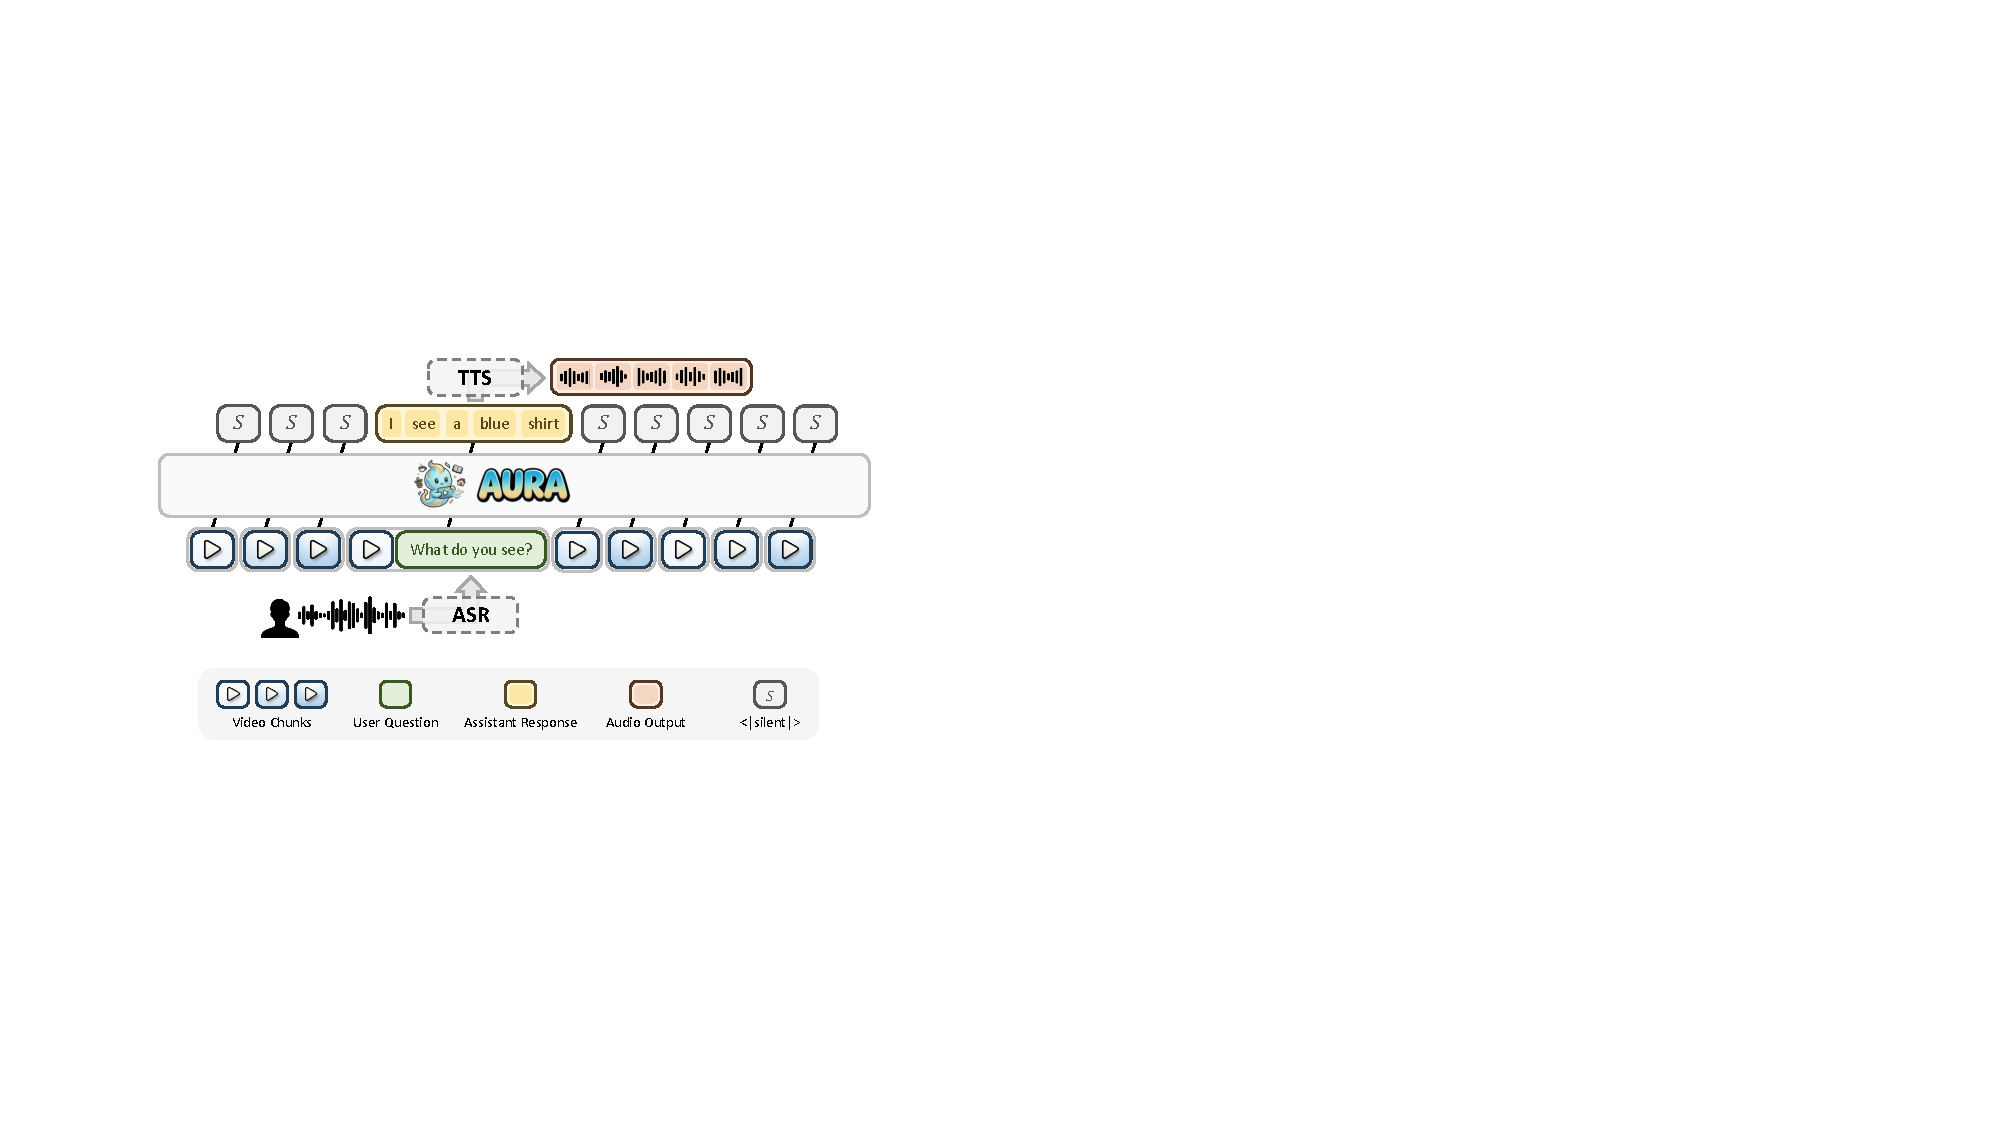
\includegraphics[width=0.95\textwidth]{img/5_inference_2.pdf}
    \caption{Overview of AURA's end-to-end real-time inference system with video and speech input, multimodal inference, and speech output. The system is designed to support continual streaming perception and low-latency interaction.}
    \label{fig:inference_pipe}
\end{figure}

To support AURA for continuous streaming perception and real-time audio-video interaction, we develop an end-to-end inference system, as illustrated in Figure~\ref{fig:inference_pipe}. The system is centered on the AURA model, integrates ASR and TTS modules, and incorporates several efficiency optimizations.

The overall context is constructed based on the Interactive Video Stream Context Management mechanism described in Section~\ref{subsec:interactive_video_stream_context_management}. On the input side, the video stream and user speech are captured simultaneously. The video stream is divided into small chunks according to a predefined chunk size. When no user speech is detected, each video chunk is independently inserted into the context as a user message. When user speech is received, it is first transcribed into text by the ASR module and then combined with the video chunk corresponding to the time at which the speech is received. The combined content is then inserted into the context as a single user message. Whenever a new user message is added to the context, the AURA model is invoked by the inference layer to generate a text response. Any non-silent response is then sent to a streaming TTS module and converted into speech, and both the text and speech are delivered to the output side. Meanwhile, the output is also added to the context as an assistant message.

% When the overall context reaches the predefined video window size $N$, context truncation is applied. A common approach is to maintain all video chunks in the context as a fixed-length first-in-first-out (FIFO) queue, removing the oldest chunk whenever a new one is added. However, this design causes the context prefix to change continuously, which prevents the reuse of previously computed KV caches (prefix caching) and significantly reduces inference efficiency. To address this problem, we adopt an improved strategy. When the window becomes full and a new video chunk arrives, we remove the oldest $N'$ video chunks at once (where $N' < N$), together with the corresponding silent assistant messages. During the insertion of the following $N'$ video chunks, no further chunks are removed, which allows the KV prefix to be reused continuously. Only when the queue length reaches $N$ again do we recompute the full video KV cache. 
% For the text QA sliding window, we do not use a separate truncation schedule. Instead, whenever video window truncation is triggered, we reduce the number of QA groups outside the video window to $M$, ensuring that the frequency of KV prefix recomputation does not increase. 
% % For the text QA sliding window, we do not maintain a separate truncation schedule. Instead, whenever the video window is truncated, we also trim the text QA groups that lie outside the video window to a maximum of $M$. This ensures that the KV prefix cache, which includes both video and text contexts, does not need to be recomputed frequently. 
% Since text tokens accumulate relatively slowly, this design also prevents the number of QA groups outside the video window from growing far beyond $M$.

Following the definition of the Interactive Video Stream Context Management mechanism, context truncation is required once the total context reaches the predefined video window size $N$. A common approach is to maintain all video chunks in the context as a fixed-length first-in-first-out (FIFO) queue, removing the oldest chunk whenever a new one is added. However, this design causes the context prefix to change continuously, which prevents the reuse of previously computed KV caches (prefix caching) and significantly reduces inference efficiency. To address this issue, we adopt an improved strategy that allows the video window to slightly extend within a margin of $N'$. Specifically, when the window size reaches $N+N'$, we remove the oldest $N'$ video chunks at once, together with the corresponding silent assistant messages. During the insertion of the next $N'$ video chunks, no further chunks are removed, which allows the KV prefix to be reused continuously. Only when the queue length again reaches $N + N'$ do we truncate the window back to $N$ by removing the oldest $N'$ video chunks, and then recompute the KV cache for the remaining $N$ chunks. For the text QA sliding window, we similarly allow it to extend slightly above $M$. However, in order to avoid increasing the frequency of KV prefix cache recomputation, we do not set a separate truncation trigger for QA. Instead, whenever the video window is truncated, we simultaneously trim the text QA groups that lie outside the video window to $M$. Since QA accumulates relatively slowly, the floating range above $M$ will also remain small. Although these two floating-window designs may cause the inference-time context length to be slightly larger than that used during training, the excess is small. In practice, we find that this design does not lead to noticeable performance degradation while significantly reducing computational cost.

Throughout the system, AURA, ASR, and TTS operate asynchronously, allowing AURA to continue running while ASR and TTS are in progress. Based on this design, we further incorporate several optimization techniques, including streaming output, computation graph optimization, and multi-process resource isolation. We also develop the frontend UI and communication protocols, resulting in a practical demo with a stable user experience that is used to evaluate AURA’s performance in real-world applications.
